\documentclass[11pt,preprint]{aastex}

\begin{document}
\def\simlt{\lower.5ex\hbox{$\; \buildrel < \over \sim \;$}}
\def\simgt{\lower.5ex\hbox{$\; \buildrel > \over \sim \;$}}

%\noindent Astronomy 121 \hfill 2004 Feb 10

\title {COMPLEX FOURIER TRANSFORMS AND SSB MIXERS \\
the week beginning March 18}

An earlier lab explored ordinary double-sideband (DSB) mixers, for which
the upper and lower sidebands produce identical mixer output. Here we
explore single-sideband (SSB) mixers, which display the remarkable
property that upper and lower sidebands produce outputs at negative and
positive baseband frequencies, respectively. In real life, SSB mixers
allow such things as the transmission and reception of stereo FM
signals; in olden days, FM transmission were all monophonic.

In that same lab we used discrete Fourier transforms (DFTs) to obtain
power spectra. We didn't look into the fundamentals of DFTs much---we
just plowed ahead. Here, it's time to study those fundamentals in some
detail from both the experimental and theoretical standpoints.

\section{GOALS}

\begin{itemize}

\item Learn how FFTs are a particular implementation of DFTs, how they
work, and what they provide.

\item Explore leakage power in DFTs.

\item Construct a two-output mixer, composed of two mixers, that can be
  operated as either a DSB or an SSB mixer. 

\item Use the two-output mixer in DSB and SSB modes and understand the
  difference. 

\item Learn how complex inputs to a FT break the negative/positive
  frequency degeneracy.

\end{itemize}


\section{THE SCHEDULE AND THE WORK}

All activities in this lab are for the week plus Spring Break, March 18 to
April Fool's day. As usual, all members of a group should do the lab work
together as a group. And all {\it analysis} should be done by {\it
  individuals}.  Important: we are working with frequency power spectra,
and all spectra should be plotted versus {\it frequency}, not channel
number! Be ready for show and tell!

\section{EXPLORING DFT/FFT}

\subsection{Leakage Power}

First, let's explore {\it Spectral Leakage}, and let's simplify things by
making the input to the DFT/FFT real so that power spectra are symmetric
about zero.  For an input signal having frequency $f_{sig}$, obtain an
input time series with $2^M$ samples, e.g.\ $M=8$ for 256 samples.  We'll
denote the Nyquist frequency by $f_N$, which is of course equal to half the
sampling frequency.

For one time series, make $f_{sig}$ equal to a multiple of $f_N \over
{2^{M-1}}$. For example, for $M=8$, there are 128 possibilities, namely
$f_{sig} = \left[ {0 \over 128},{f_N \over 128},{2 f_N \over 128},{3 f_N
    \over 128},{4 f_N \over 128}, \dots {127 f_N \over 128}\right]$, so you
have plenty of choices (some of which aren't reasonable\dots). Pick 1 or 2,
take the data, and calculate the power spectrum. Turn up the vertical scale
a lot to see if there is any nonzero power at frequencies other than
$f_{sig}$.

So much for $f_{sig}$ being integral multiples of $f_N \over
2^{M-1}$. How about half-integral multiples? Again, try one or
two---e.g. $f_{sig} = \left[ {0.5 f_N \over 128},{1.5 f_N \over
128},{2.5 f_N \over 128}\dots \right]$.  Again, turn up the scale on the
power spectrum. What's the difference between the above result and this
one?

This is {\it Spectral Leakage}. It affects all power spectra calculated
using Fourier techniques. Can you understand what's going on from a
mathematical viewpoint?

\subsection{More Leakage Power!} \label{leakage}

So there's {\it no} leakage power for $f_{sig}$ being integral multiples of
$f_N \over 2^{M-1}$? Think again! From your first time series above (the
one that has $f_{sig}$ an integral multiple of $f_N \over 2^{M-1}$),
calculate the power spectrum at frequencies much closer together than $f_N
\over 2^{M-1}$, maybe 8 or 10 times closer. For example, for $M=8$ you'd
usually calculate $2^M=256$ points for the power spectrum between $-f_N$
and $+f_N$; try calculating 2048 or 2560 points, or some other large
number. (For this you need to use the {\tt dft} procedure, not {\tt fft}).
Do you see leakage? Again, can you understand what's going on from a
mathematical viewpoint?

\subsection{Frequency Resolution}

If you had two sharp spectral lines, how closely spaced in frequency
could they be and still resolve them? Roughly, this is just the apparent
width of the line when plotted against frequency. Look at the width of
the line for your plot of \S \ref{leakage} above. Compare this width to
$1 \over T$, where $T$ is the total time span over which the samples
were taken. If you have the inclination, try taking other time series
with varying number of samples (and thus, varying $T$) and confirm any
relationship between line width (that is, frequency resolution) and
$T$. 




\section{ CONSTRUCT A TWO-OUTPUT MIXER USABLE FOR DSB OR SSB}
\label{upperlowerdsb}

From the block diagram given below in Figure \ref{ssbmfig} and in class,
construct a ``Computer Voodoo'' SSB mixer that achieves the phase delay
with a cable instead of a quadrature hybrid. We will use it to experiment
with no phase delay (a short cable) and a 90-degree phase delay (a long
cable).

For experimentation with this two-output mixer, use two SRS synthesizer
oscillators as inputs.  The SRS synthesizers work up to 30 MHz.  Assign
one of the SRS synthesizers to be your ``local oscillator'' with
frequency $f_{lo}$, and the other your ``signal'' with frequencies $f_{sig}
= f_{lo} \pm |\delta f|$.  To prevent aliasing and to filter out the sum
frequency, we will use the 5-MHz low-pass filters, one on each output of
the two-output mixer. Thus, we will want $|\delta f| < 5$ MHz. Moreover,
remember the Nyquist criterion: we want to see mixing products up to at
least 5 MHz, so you'll need to sample\dots at least how often?

The computer's ADC samples the two outputs simultaneously. We use the
two outputs as inputs to the DFT---one as the real, the other as the
imaginary input.

\section{THE DSB MIXER} \label{dsbmixer}

First see what happens when the phase delay cable is short, so that the two
outputs have no relative phase delay. Pick a value for $|\delta f|$ and
take time series data for the two corresponding values of $f_{sig}$ (these
are the upper and lower sidebands). Calculate the power spectra. When
taking the Fourier transform, be sure to make the inputs complex---you have
two simultaneous samples, one real and one imaginary. Looking at the power
spectra alone, can you distinguish between positive and negative $\delta
f$?


\section{THE SSB MIXER---EXPERIMENT}

Now see what happens when the phase delay cable introduces a relative phase
delay of $90^\circ$ between the l.o.\ signals going to the two mixers.
Repeat what you did above in \S \ref{dsbmixer}. Looking at the power
spectra alone, can you distinguish between positive and negative $\delta
f$?

If you have the time and inclination, verify that the phase difference
between the two mixer outputs behaves as shown in Figure \ref{dsbmixer}.
Why does it behave this way?  (Look at equations \ref{rhs} and \ref{lhs} in
\S \ref{mathdescr}.)

We could repeat the experiments on spectral leakage for the SSB case, but
we'd find the same kind of results as we did for DSB, so don't bother
unless you're really gung-ho.

\section{THE SSB MIXER---THEORY}

The SSB mixer has the capability of distinguishing whether the
difference frequency $|\delta f|$ is positive or negative---that
is, it distinguishes between the two sidebands.  The sidebands can, and
usually do, contain completely independent signals. The SSB mixer has
two outputs, one for each sideband.

        These signals really are completely independent. For example, FM
broadcasts are usually done in stereo and one could transmit the left
and right hand channels in the two sidebands; in fact, for a variety of
reasons, it's done differently, with the upper sideband carrying the sum
of the left/right channels and the lower sideband the difference.

\begin{figure}[p!]
%\leavevmode
%
%\begin{center}
\hspace{-0.75in}
\includegraphics[width=7.5in, height=8.0in]{sideband.ps}
%\end{center}
\caption{Upper and lower sidebands in DSB and SSB mixers for a set of
$\delta$-function test signals on top of broad level noise spectra. Top:
the RF spectrum. The next two show the USB and LSB {\it individually}
when they undergo the DSB mixing process; panel 4 shows how they both
add together. The bottom panel shows the SSB mixer, which keeps them
separate. \label{sideband}}
\end{figure}

Figure \ref{sideband} illustrates this crucial element. It considers
DSB and SSB mixers that are converting RF to baseband and compares the
the responses to upper and lower sidebands (USB and LSB). The top panel
shows the original RF spectrum. The second panel shows the USB after DSB
mixing: it appears at {\it both} negative and positive frequencies in
the output spectrum so that the output baseband spectrum is symmetric,
meaning that the negative frequencies give exactly the same result as
the positive ones. The third panel shows the same for the LSB. You can
achieve the rejection of either the LSB or the USB by using an
appropriate {\it bandpass} filter at RF. The fourth panel shows what
happens without a bandpass filter: with independent, different LSB and
USB inputs, the LSB and USB are inextricably mixed in the output
spectrum and you get the sum of the two power spectra. The bottom panel
shows that SSB (Single Sideband) mixing retains the sideband separation
and identity.



\subsection{A Preliminary: The Quadrature Hybrid}

        The heart of a SSB mixer is not the mixer. Rather, it's the
quadrature hybrid. So before considering SSB mixers, we need to
understand hybrids and quadrature hybrids\footnote{For an excellent and
thorough discussion of hybrids and their applications, refer to:  Hagen,
Jon B., ``Radio-Frequency Electronics, Circuits and Applications,''
Cambridge University Press, 1996, pg. 188-200.}.


\begin{figure}[!h]
\begin{center}
$\begin{array}{cc}
        \includegraphics[width=2.0in]{hybrid1.plt}
        &
        \includegraphics[width=2.0in]{hybrid2.plt}
        \\
        \parbox[t]{3.0in}{\caption{Block diagram of a four port hybrid.
\label{hybrid1}}}\hspace{0.4in}        &
        \parbox[t]{3.0in}{\caption{Block diagram of a quadrature hybrid.
\label{hybrid2}}}
\end{array}$
\end{center}
\end{figure}


        Figure\ \ref{hybrid1} shows the block diagram of a hybrid.  The
signal acts just like the diagram shows: a signal entering port\ 1 will
split into equal signals (--3 dB each) and exit through ports\ 2 and 3.
No power is transmitted across the hybrid to port\ 4.  Internally, many
hybrids look like center-tapped transformers; see Hagen's book.

        Power is split between the two adjacent ports and nothing is
transmitted across it.  In this way we think of a hybrid as a {\it power
splitter}.  In fact, this is just what power splitters are: a hybrid
with the fourth port terminated in a matched load. If you are wondering
if it can be used in reverse as a power combiner, the answer is yes.  If
inputs are made to ports\ 1 and 4, the sum of the inputs exit through
ports\ 2 and 3. One point: all ports must present matched loads. By
symmetry, ports 2 and 3 each get half the power, so if one of these is
terminated then half the power is lost\footnote{Unless the combining
  signals are identical with a particular phase relationship, in which
  case all of the power can go to the unterminated port.}.

        Hybrids can be made so that they add a phase angle, either
$90^\circ$ symmetrically in two legs or $180^\circ$ in one leg.
Figure\ \ref{hybrid2} shows a block diagram.  A signal incident on port\
1
splits and exits through ports\ 2 and 3, but  each signal is
\emph{shifted} by the number of degrees specified in each corner of the
schematic:  the output of port\ 2 is shifted by $90$ degrees with
respect to the input while the
output of port\ 3 is not shifted at all.


\subsection{The SSB mixer: block diagram and graphical description}

\begin{figure}[ht]
        \begin{center}
        \leavevmode
        \includegraphics[width=3in]{ssbmix.plt}
        \end{center}
        \caption{Block diagram of the all-hardware and
                hardware/software combination SSB mixer. In the lab,
                we'll replace the upper quadrature hybrid with a
                $\lambda \over 4$ length of cable.}\label{ssbmfig}
\end{figure}

Figure\ \ref{ssbmfig} shows a block diagram of the SSB mixer.  The RF
input is split by a power splitter into two equal channels. The LO is
split by a hybrid, so that the left hand side (LHS) leads the RHS by
$90^\circ$.  These two channels are recombined with the second
quadrature hybrid.

We kind of lied above when we said that the quadrature hybrid is the
heart of the SSB mixer. The function of the first (top) hybrid is to
produce a $90^\circ$ phase shift between the two l.o.\ signals going to
the two mixers. We could generate this phase shift in another way:
replace the quadrature hybrid with an ordinary power splitter, and, in
one leg, a cable of appropriate length (which would, of course, be
$\lambda \over 4$).

        Suppose that the signal ``RF in'' is a cosine wave in the lower
sideband, with frequency below the l.o.\ frequency. The l.o.\ is a
cosine wave on the RHS and a sine wave on the LHS (because of the
$90^\circ$ shift). This makes the two mixer outputs
$\propto \sin [\delta \omega t]$ and $\cos [\delta \omega t]$ for the
LHS and RHS, respectively. These are shown in Figure \ref{mixerout},
with the LHS side [$MO(LHS)_-$] dashed and the RHS [$MO(RHS)_+$]
solid. These are identical in amplitude: they have to be, because they
come from the same original lower-sideband signal. But they are shifted
in phase: the dashed curve lags behind the solid one.

\begin{figure}[h]
%        \begin{center}
\hspace{-0.5in}
%        \leavevmode
        \includegraphics{ssbm.ps}
%        \end{center}
        \caption{Outputs of the first mixers for the two sideband
	  cases---USB ($\delta f > 0$) on the left, LSB ($\delta f< 0$) on
	  the left.  Dashed is the left-hand mixer (LHS), solid is
	  right-hand mixer (RHS).
\label{mixerout}}
\end{figure}



        Now suppose we shift the {\it dashed} curve forward by
$90^\circ$; then it {\it adds} constructively with the solid curve and
gives twice the amplitude. Alternatively, suppose we shift the {\it
solid} one forward by $90^\circ$; then the two signals {\it cancel}.

How do we do this $90^\circ$ phase shifting? We can do it
digitally, by taking its Fourier transform with the two inputs being the
real and imaginary components of the input numbers (which are complex).
Or we can do it with another
$90^\circ$ hybrid! 

\subsection{The Digital ``Computer Voodoo'' Method}

In Figure \ref{ssbmfig}, we can regard the two independent signals
marked ``To ADC for Computer Voodoo'', as as the real and imaginary
components of the signal because, no matter what the input frequency,
they differ in phase by $90^\circ$. So the signal is a complex
number. With an ordinary DSB mixer the signal is a real number, so its
Fourier transform must have Hermitian symmetry---meaning that the power
spectrum is symmetric, with negative and positive frequencies being
identical. Here, the signal is a complex number, and there is no
symmetry. We won't delve into the math here, but the net result is that
the Fourier transform keeps the negative and positive frequency
components completely separate. Real geeks call this method ``QU
sampling''. 

\subsection{The Analog method}

You don't have to do it digitally. In Figure \ref{ssbmfig}, the second
quadrature hybrid at the bottom does exactly this combination of
functions! So a lower-sideband signal comes out of the LSB port, and an
upper-sideband one comes out of the USB port. The phase combining is
linear, so if there exist, simultaneously, different signals in the two
sidebands, their separation is maintained at the output. Technically,
it's not easy to make a quadrature hybrid that operates at baseband, so
when operating at baseband the ``Computer Voodoo'' method is more
common. 



\subsection{Mathematical description} \label{mathdescr}

        First, we mix the incoming signal with the real and imaginary
(cosine and sine) components of the l.o. As in the DSB mixer, we use a
low pass filter so we need consider only the difference frequencies. For
the left hand side the l.o.\ has the $90^\circ$ phase difference so it's
a $\sin$ instead of a $\cos$ and for the Mixer Output ($MO$) we have

\begin{equation}
MO(LHS)_\pm = {E_s \over 2} \sin [\pm|\delta \omega | t]
\end{equation}

\noindent so, writing the results separately for the two sidebands as we
did above, we have

\begin{mathletters} \label{rhs}
\begin{equation}
MO(LHS)_- = {E_s \over 2} \sin [-|\delta \omega | t] =
   -{E_s \over 2} \sin [|\delta \omega | t]
\end{equation}
\begin{equation}
MO(LHS)_+ = {E_s \over 2} \sin [+|\delta \omega | t] =
   {E_s \over 2} \sin [|\delta \omega | t]
\end{equation}
\end{mathletters}

\noindent Similarly, for the RHS we have

\begin{mathletters} \label{lhs}
\begin{equation}
MO(RHS)_- = {E_s \over 2} \cos [-|\delta \omega | t] =
   {E_s \over 2} \cos [|\delta \omega | t]
\end{equation}
\begin{equation}
MO(RHS)_+ = {E_s \over 2} \cos [+|\delta \omega | t] =
   {E_s \over 2} \cos [|\delta \omega | t]
\end{equation}
\end{mathletters}

\noindent The RHS and LHS outputs have identical frequencies and
amplitudes.


        {\it But the phase relationships differ for the two sidebands.}
For the {\it lower} sideband, the RHS output {\it lags} the LHS by
$90^\circ$; for the {\it upper} sideband, the RHS output {\it leads} the
LHS by $90^\circ$, just as in Figure \ref{mixerout}. In other words, for
the RHS output, lower-sideband signals differ in sign from
upper-sideband ones; this is equivalent to differing in phase by
$180^\circ$.

        In the second half of the SSB mixer the signals are recombined
in a second $90^\circ$ hybrid. Referring to Figure \ref{ssbmfig}, the
LSB (lower sideband) output is equal to the sum of RHS plus LHS delayed
by $90^\circ$, conveniently written

\begin{mathletters}
\begin{equation}
MO(LSB) = MO(LHS) + MO(RHS) \angle 90^\circ
\end{equation}

\noindent In contrast, the USB output is
\begin{equation}
MO(USB) = MO(LHS)\angle 90^\circ + MO(RHS)
\end{equation}
\end{mathletters}

\subsection{Lower sideband output}

        Now consider the lower sideband output $MO(LSB)$. For the {\it
lower sideband signal} of frequency $(\omega_0 - |\delta \omega|)$, the
relevant quantities are $MO(LHS)_-$ and $MO(RHS)_- \angle 90^\circ$.
These are just

\begin{mathletters}
\begin{equation}
MO(LHS)_- =
-{E_s \over 2} \sin [|\delta \omega | t]
\end{equation}

\begin{equation}
MO(RHS)_- \angle 90^\circ =
{E_s \over 2} \cos [|\delta \omega | t + 90^\circ] =
   -{E_s \over 2} \sin [|\delta \omega | t]
\end{equation}
\end{mathletters}

\noindent Adding them gives $MO(LSB)_-$, so we have


\begin{mathletters}
\begin{equation}
MO(LSB)_- = MO(LHS)_- + MO(RHS)_- \angle 90^\circ =
   -E_s  \sin [|\delta \omega | t]
\end{equation}

\noindent If we carry through the same algebra for the {\it upper
sideband signal} of frequency $(\omega_0 + |\delta \omega|)$, we get

\begin{equation}
MO(LSB)_+ = MO(LHS)_+ + MO(RHS)_+ \angle 90^\circ = 0
\end{equation}
\end{mathletters}

\noindent So we see that the LSB output {\it excludes the positive
frequencies} (upper sideband), as promised.

\subsection{Upper sideband output}

        We can go through the identical steps for the USB output. We
then obtain

\begin{mathletters}
\begin{equation}
MO(USB)_- =  MO(LHS)_- \angle 90^\circ  + MO(RHS)_- = 0
\end{equation}

\begin{equation}
MO(USB)_+ = MO(LHS)_+   \angle 90^\circ + MO(RHS)_+ =
        E_s  \cos [|\delta \omega | t]
\end{equation}
\end{mathletters}

\noindent and the USB excludes the lower sideband.



\section{AN ASIDE: COMPLEX NOTATION AND POSITIVE/NEGATIVE FREQUENCIES}
\label{complex}

        Remember the relationship between trig functions and complex
exponentials:
                                                                        
       
\begin{mathletters} \label{cossin}
\begin{equation}
\sin(\omega t) = {1\over 2j} [\underbrace{\exp(+j\omega t)}_{pos\ freq}
        - \underbrace{\exp(-j\omega t)]}_{neg\ freq}
\end{equation}
\begin{equation}
\cos(\omega t) = {1\over 2} [\underbrace{\exp(+j\omega t)}_{pos\ freq}
        + \underbrace{\exp(-j\omega t)]}_{neg\ freq}
\end{equation}
\end{mathletters}
                                                                        
       
\noindent This means that any sine wave can be considered as a
superposition of two frequencies, one positive and one negative; ditto
for a cosine wave. We can speak of the ``negative frequency branch'' and
the
``positive frequency branch''.
                                                                        
       
        What's this ``negative frequency'' business---is it just a
mathematical construction? {\it NO!!!!} Consider a rotating wheel: cars
can go backwards as well as forwards. The wheel rotates $\omega \over
2\pi$ times per second; one direction is positive frequency, one is
negative.


        Suppose we rewrite equation \ref{cossin} in complex form, in
which the cosine and sine terms are real and complex. This gives

\begin{mathletters} 
\begin{equation}
	MO_{complex, \pm} = MO_{cos, \pm} + j MO_{sin, \pm} 
\end{equation}
\noindent or,  %from equation \ref{baseband}
\begin{equation}
	MO_{complex, \pm} = {E_s \over 2} [ \cos ( |\delta \omega | t )
+ j \sin ( |\delta \omega | t )]
\end{equation}
\noindent or the convenient shorthand form
\begin{equation}
	MO_{complex, \pm} = {E_s \over 2} e^{2 \pi j |\delta \omega| t} \ .
\end{equation}
\end{mathletters}

\end{document} 

